\documentclass{mathrep}

\newcommand{\xelatexemojipath}[1]{./apple-emoji/png/160/emoji_u#1.png}
\usepackage{xelatexemoji}
% \usepackage{darkmode}
% \enabledarkmode

\usepackage{layout}

\title{Compilation}
\date{\today}
\author{雅思数论}

% \includeonly{
%   ./chapter/collision_and_pi
% }

\begin{document}

\frontmatter
\maketitle

% \chapter*{Preface}
% \addcontentsline{toc}{chapter}{\protect\numberline{}Preface}

\tableofcontents

\mainmatter
\chapter{康托尔集合论:无穷的性质}

\section{无穷集合的比较}
\subsection{引入}
想必大家一定听说过有名的无限旅馆的故事.

\paragraph{希尔伯特旅馆}
有一家无限间房间的旅馆, 但旅馆已经满客.
此时来了一位客人想要入住, 老板说:“没问题!”
老板安排1号房客人挪到2号房, 2号房挪到3号房, 3号房挪到4号房, 以此类推.
结果是1号房空出来了, 新客人可以入住了.
而这时又来了无穷多的客人, 老板又说:“没问题!”
然后老板发布通知, 每个客人都挪到自己房间号两倍的房间, 这样奇数号房间都空出来了, 无穷多的客人可以入住了.

这个故事看似荒诞不经, 但并非毫无道理, 其与无穷集合的比较有关.

\subsection{定义}
\label{defi}
假设我们并不认识$3$以上的数字, 那么我们要怎么比较$7$枚铜币和$8$枚铁币呢?
其实我们可以将铜币和铁币一个一个拿出, 每次各拿一个, 最后剩下哪一种币, 就是哪一种数量多.
同样, 我们可以用这种方法比较无穷集合的大小, 如偶数集与奇数集的元素个数一样多:
\begin{table}[!ht]
  \begin{center}
    \begin{tabular}{c|lllll}
      \toprule
      $\mathrm O$ & 1 & 3 & 5 & 7 & $\cdots$ \\
      \midrule
      $\mathrm E$ & 2 & 4 & 6 & 8 & $\cdots$ \\
      \bottomrule
    \end{tabular}
    \caption{奇数与偶数一一对应}
  \end{center}
\end{table}

虽然可能有点颠覆认知, 但是通过这种方法, 我们得出了正整数集与偶数集一样大的结论.

\begin{table}[!h]
  \begin{center}
    \begin{tabular}{c|lllll}
      \toprule
      $\mathrm N_+$ & 1 & 2 & 3 & 4 & $\cdots$ \\
      \midrule
      $\mathrm O$   & 2 & 4 & 6 & 8 & $\cdots$ \\
      \bottomrule
    \end{tabular}
    \caption{正整数与偶数一一对应}
  \end{center}
\end{table}

同样, 正平方数集与正整数集一样大.

\begin{table}[!h]
  \begin{center}
    \begin{tabular}{c|lllll}
      \toprule
      $\mathrm N_+$ & 1 & 2 & 3 & 4  & $\cdots$ \\
      \midrule
      $n^2$         & 1 & 4 & 9 & 16 & $\cdots$ \\
      \bottomrule
    \end{tabular}
    \caption{奇数与偶数一一对应}
  \end{center}
\end{table}

那如果两个无穷集合无法一一对应, 那如何比较谁大谁小呢?

\begin{definition}
  若集合$A$与$B$无法建立一一对应, 且$B$的一个子集为$C$(同样也是无穷集合), $C$能够与$A$建立一一对应关系, 则$B$比$A$大.
  记为$\abs{B} > \abs{A}$.
\end{definition}

\section{正整数集与有理数}

了解以上定义之后, 我们是时候研究一下各无穷集合之间的关系了,
那我们先来会会我们的老朋友正整数集$\mathbb N_+$与有理数集$\mathbb Q$.
有理数集看似远远大于正整数集, 但是不要被表象迷惑, 他们俩之间存在一种巧妙的对应关系.

\begin{figure}[htbp]
  \begin{center}
    \includegraphics[scale=1]{natural-rational-bijection}
    \caption{自然数与有理数的一一对应}
    \label{fig:bijection}
  \end{center}
\end{figure}

如 \cref{fig:bijection}, 我们制出一个关于有正有理数的表, 我们可以肯定里面肯定包括了所有的正有理数,
按照红线将其拉长成1条直线, 再去掉重复的项,
我们就得到了一个正有理数的集合, 可以用这样的排列方法将有理数与正整数一一对应.
\footnote{编者按:即有理数集是可数集. }

但是这个集合只是与正有理数等大, 而不是与有理数等大.
所以我们要运用无限旅馆中的技巧.
我们将正整数分为三部分:

\begin{enumerate}
  \item \label{enum:1} ${1}$
  \item \label{enum:2} 偶数
  \item \label{enum:3} 除$1$以外的偶数
\end{enumerate}

将\cref{enum:1}与$0$对应,
将\cref{enum:2}与新的正整数$\mathbb N_+$对应,
再按如上方法与正有理数对应.
如下:

\begin{table}[h!]
  \begin{center}
    \begin{tabular}{c|lllll}
      \toprule
      $\mathrm N_+$ & 1 & 2             & 3 & 4 & $\cdots$ \\
      \midrule
      $\mathrm O$   & 2 & 4             & 6 & 8 & $\cdots$ \\
      \midrule
      $\mathrm Q_+$ & 1 & $\frac{1}{2}$ & 2 & 3 & $\cdots$ \\
      \bottomrule
    \end{tabular}
    \caption{间接对应}
  \end{center}
\end{table}

而\cref{enum:3}也一样, 先与一个新的整数集\footnote{编者注:此处应该为奇数集}对应, 再与负有理数集$\mathbb Q_-$对应.
这样正整数集的三部分就分别对应了有理数的$0$、正、负三部分, 我们得到了正整数与有理数等大的结论.

\subsection{幂集}
\label{ssec:powerset}
我们在 \cref{defi} 中说到,
无法互相一一对应的无穷集合, 可能会有人质疑存在这样的集合吗?
其实, 这一方面的奠基人康托尔
\footnote{编者注: Cantor,Georg Ferdinand Ludwig Philipp,
  1845年3月3日--1918年1月6日.
集合论的创始人, 最早从事无穷集合的一般理论研究的数学家. }
已经为我们发明了一种工具:幂集.

\begin{definition}[幂集(power set)]
  给定集合$A$ , 记$2^{A}$为集合 $A$  的子集的集合, 即 $2^{A}=\{ X|X\subset A \}$. 称
  $2^{A}$ 是 $A$ 的\textbf{幂集(power set)}.
  \footnote{编者注:这里不同于原文, 采用了一种更加常见的记法. },
\end{definition}

如果$A=\{1, 2, 3\}$ , 那么就有
\[
  2^A=\{\varnothing, \{1\}, \{2\}, \{3\}, \{1, 2\}, \{1, 3\}, \{2, 3\}, A\}
.\]
注意空集 $\varnothing$ 和 $A$本身都是 $2^{A}$ 的元素, 取子集的时候不要忘了空集和集合本身.
\footnote{由于无穷集合的幂集难以用列举法表示此处用有限集来举例. }

集合和幂集的基数之间有什么关系呢?

答案是 $\abs{2^A} =2^{ \abs{A} }$, 这也是把幂集记为 $2^A$ 的主要原因.
对于有限集合 $A$, 显然有 $\abs{2^A} =2^{ \abs{A} }> \abs{A}$,
那么对于无限集合 $B$ 会怎样呢?都是无限, $\abs{B}$ 和 $\abs{2^B}$ 相等吗?

答案是否定的, 因为不存在 $B$ 到 $2^B$ 的一一对应\footnote{编者注:此处应为满射. 如果 $f: A \to B$
中每个 $B$ 中元素都至少被$A$中的一个元素所对应, 那么称 $f$ 是一个\textbf{满射(surjection)}. },
按照定义, 这就是说, $\abs{2^B}$ 严格大于 $\abs{B}$.

\begin{proof}
  设$A= \{a,b,c,d,\cdots\}$($A$中的元素不局限于数字).
  假设$A$与$2^{A}$存在对应关系.
  例如:
  \begin{table}
    \begin{center}

      \begin{tabular}{ccc}
        \toprule
        $A$      & ~                 & $2^{A}$                  \\
        \midrule
        $a$      & $\leftrightarrow$ & $\{a,\theta ,\varphi \}$ \\
        $b$      & $\leftrightarrow$ & $\varnothing$            \\
        $c$      & $\leftrightarrow$ & $\{m,n,o \ldots \}$      \\
        $\ldots$ & $\leftrightarrow$ & $\ldots$                 \\
        \bottomrule
      \end{tabular}
      \caption{元素与其幂集的子集的对应关系}

    \end{center}
  \end{table}
  则发现, 左边$A$中的元素可分为两类:
  \begin{enumerate}
    \item \label{enum:in}属于其右边对应的集合(A的子集之一)
    \item \label{enum:notin}不属于其右边对应的集合
  \end{enumerate}
  那么\cref{enum:notin}中的元素就可以构成一个集合.
  设为集合$T$. 因为$T\subset A$, $T \in 2^{A} $.
  所以$T$也有一个对应的$A$中的元素, 设为$t$.

  所以
  \begin{enumerate}
    \item 若$t \in T$, 则 $t$ 是 \cref{enum:in} 所指的元素, 而 \cref{enum:in}
      的元素并没有被归入 $T$, 所以 $t \not\in T$, 矛盾.
    \item 若$t \not\in T$, 则 $t$ 是 \cref{enum:notin} 所指的元素, 所以 $t$
      被归入了 集合$T$, 得到 $t \in T$, 矛盾.
  \end{enumerate}

  结果就是, 无论以哪种方法对应, 总存在这样的集合$T$, 使得没有$A$中的元素与其一一对应.
  所以$A$与$2^{A}$无法一一对应.
  但是$2^{A} $的子集能与$A$对应. (不妨取这样的子集$ \{ \{a\},\{b\},\{c\}, \ldots \}
  $显然能与$A = \{a, b, c, d, \ldots \} $一一对应).

  所以$\abs{2^{A}}> \abs{A}$.

\end{proof}

\subsection{
  \texorpdfstring{$\left[ 0, 1 \right]$与$2^{\mathbb{N}_+}
  $与$\mathbb{R}$上的任意点}{[0, 1]与2\^N+与R上的任意点}
}
在我们证明完 $2^{A}>A$之后, 我们想到:$2^{\mathbb{N}_+} $太难理解了,
有没有什么直观的集合跟他等势
\footnote{我们把集合所包含的元素数量称作\textbf{基数}(cardinal, 或\textbf{势}).
用这个术语来说, 比较集合的大小就是在比较它们的基数的大小. }
呢.

有的兄弟, 有的. 就是$\left[0, 1\right]$.

\begin{note}[任意进制的数字表述] \label{note:system_of_numeration}
  在任意进制的数字表示中,
  小数点前第$n$位表示的是该进制基数的$n-1$次方,
  小数点后第$n$位表示的是该进制基数的$-n$次方.

  例如: 在十进制的$123. 4$中, 个位数的3表示$3 \times 10^{0} $,
  十位数的2表示$2 \times 10^{1} $,
  百位数的1表示$1 \times 10^{2} $,
  而十分位数的4表示$4 \times 10^{-1} $.

  我们将n进制数标记为右上角的「$^{(n)}$」, 例如我们将二进制数$11010$记为$11010^{(2)}$
\end{note}

让我们将$\left[ 0, 1 \right]$中的小数记为二进制.
不妨记 $1^{(10)} $ 为$0. 1111\ldots ^{(2)} $
记$0^{(10)} $为 $0. 0000\ldots ^{(2)} $.

\begin{note}[$0. 1111\ldots ^{(2)}  $等于$1^{(10)}$]
  由\cref{note:system_of_numeration}我们得知
  \begin{align*}
    0. 1111\ldots ^{(2)} & = \sum_{n=1}^{\infty} \frac{1}{2^{-n}}          \\
    & = \frac{1}{2}+\frac{1}{4} +\frac{1}{8} + \ldots \\
    & = 1
  \end{align*}
  不妨类比为$0. 999\ldots ^{(10)} = 1 ^{(10)} $
\end{note}

因为$2^{\mathbb{N}_+} $的元素是正整数构成的集合或者$\varnothing$,
我们不妨构造这样一个对应关系:属于$\left[0, 1\right]$的二进制小数, 若小数点后第$n$位是$1$,
则我们将$n$放入其对应的集合, 若为零则反之.

\begin{table}
  \begin{center}
    \begin{tabular}{lcc}
      \toprule
      $0. 0000\ldots $               & $\leftrightarrow$ &
      $\varnothing$                                                 \\
      $0. 01101$                     & $\leftrightarrow$ & $\{2, 3,
      5\}$                                                          \\
      $0. 101100111000\ldots $ (无理数) & $\leftrightarrow$ & $\{1, 3,
      4, 7, 8, 9,\ldots \}  $                                       \\
      $0. 1111\ldots $               & $\leftrightarrow$ &
      $\mathbb{N}_+$                                                \\
      \bottomrule
    \end{tabular}
    \caption{[0, 1]的小数与自然数幂集的子集的对应关系}
    \label{tbl:01to2N}
  \end{center}
\end{table}

\begin{figure}
  \begin{center}
    \includegraphics{tan01toR}
    \caption{函数图像} \label{fig:tan}
  \end{center}
\end{figure}

例如 \cref{tbl:01to2N},
我们得到了$\left[0, 1\right]$与$2^{\mathbb{N}_+} $ 等势的结论.

我们又有一个明确的函数, 使$\left(0, 1\right)$与$\mathbb{R}$ 一一对应, 如\cref{fig:tan}
\begin{align}
  f \colon (0, 1) \to \mathbb{R} \colon f(x) = \tan (\pi x -
  \frac{\pi}{2}) \label{fn:tan01toR}
\end{align}

再运用无限旅馆的小技巧, 则有
\[
  2^{\mathbb{N}_+}\leftrightarrow [0, 1] \leftrightarrow (0, 1)
  \leftrightarrow \mathbb{R}
.\]

Amazing! $\abs{2^{\mathbb{N}_+}} = \abs{R}$ !

我们还能证明他们与平面上所有的点的集合$\mathbb{R}^{2} = \{(x,y)| x, y \in R\} $等势.

\begin{proof}

  取任意 $x \in (0, 1)$, 分离$x$的奇数位与偶数位, 按照原来的顺序排成两个新的小数,
  不妨让奇数位组成的小数为横坐标, 偶数位为纵坐标, 组成有序数对.

  例如:
  \[
    0. 114514 \leftrightarrow (0. 141, 0. 154)
  .\]
  从\cref{fn:tan01toR}我们可以构造函数 $g(a,b)$:
  \[
    g \colon \{(a,b) | a, b \in (0, 1) \}  \to \mathbb{R}^{2}  \colon
    g(a,b) = (f(a), f(b))
  .\]
  所以有
  \[
    [0, 1] \leftrightarrow \{(a,b)| a,b \in [0, 1]\} \leftrightarrow
    \mathbb{R}^{2}
  .\]
  所以任意二维有序数对(向量)所组成的集合与$2^{\mathbb{N}_+} $ 等势.
\end{proof}

同样地, 我们可以证明任意$n$维有序数对的集合与$2^{\mathbb{N}_+} $等势. 读者自证不难.

\subsection{\texorpdfstring{$\aleph $: Aleph 基数}{Aleph 基数}}

在\cref{ssec:powerset}中, 我们知道了一个无穷集的幂集一定大于这个无穷集自身. 所以这世上没有最大的集合, 只有更大的.
就像我们可以给实数排序一样, 我们也可以给无穷集按照基数大小排序.

我们用希伯来字母$\aleph$ (Aleph, 阿列夫) 来表示无穷大, 用下标表示级别. $\aleph_0 = \abs{\mathbb{N}}$
$\aleph_1 = \abs{\mathbb{R}}$.

\begin{definition}[无穷基数]
  若$\aleph_n =\abs{A}$, 那么 $\aleph_{n+1} = \abs{2^{A} }$
\end{definition}

\subsection{连续统假设}

\paragraph{连续统猜想(Continuum Hypothesis)}
康托尔研究集合论时提出
在可列集基数$\aleph_0$和实数基数$\aleph_{1}$之间没有别的基数, 这就是著名的连续统假设. 它又被称为希尔伯特第一问题.

\begin{note}
  18世纪70年代, 康托尔在研究无穷集的势时,
  首次发现不同的无穷可以具有不同的基数.
  自然数集的势被记作$\aleph_{0}$, 而实数集的势, 称为“连续统”, 记作 $\aleph_{1}$.

  康托尔提出一个问题:是否存在一个集合, 其基数严格大于 $\aleph_{0}$ 而小于 $\aleph_{1}$?这就是连续统假设(CH).
  也就是$2^{\aleph_0}$是否等于$\aleph_0$的继承者(successor), $\aleph_1$.

  康托尔猜想了$2^{\aleph_0}=\aleph_1$, 这就是
  ---因为希尔伯特将其放在他于1900年发表的一些重要而尚未解决的问题
  \footnote{希尔伯特(David Hilbert, 1862年1月23日--1943年2月14日,
    在一些历史著作中, 他与阿基米德、牛顿和高斯等重要数学家齐名, 被誉为“数学王子”)
    在1900年将连续统假设列为他提出的23个重要的数学难题中的第一题,
  标志着这一问题地位的确立. 它触及数学最根本的基础:形式系统是否有能力决定所有陈述的真假. }
  中, 而变得十分著名的---
  连续统猜想.
  其答案是连续统猜想是无法被判定的(undecidable).
\end{note}

哥德尔
\footnote{库尔特·哥德尔(Kurt Gödel, 1906年4月28日—1978年1月14日),
美籍奥地利数学家、逻辑学家和哲学家, 是二十世纪最伟大的逻辑学家之一, 其最杰出的贡献是哥德尔不完全性定理. }
证明了公理系统的\textbf{不完备性}---每个数学系统都存在一些命题永远无法被证明真伪.
这被称为\textbf{哥德尔不完备定理}.

再由保罗·寇恩
\footnote{保罗·寇恩(Paul Joseph Cohen, 1934年4月2日---2007年3月23日), 美国数学家,
凭借连续统假设的独立性证明于1966年获得菲尔兹奖章. }
用力迫法证明了连续统假设的不可判定性.

\paragraph{习题}
证明无穷集合$A$与其有穷子集组成的集合等大, 即
\[
  \abs{A} = \abs{ \{ B| B \subset A, \abs{B} \in \mathbb{N} \}  }
.\]

% paragraph infty_hotel  (end)

\chapter{初探微积分}

\section{高等数学之门---抛物线下的面积与微积分}

\begin{figure}
  \centering
    \documentclass[border=3pt]{standalone}
\usepackage{tikz}
\usepackage{amsmath}
\usepackage{amssymb}
\usepackage{ctex}
\usetikzlibrary{matrix, calc, positioning}
\usepackage{pgfplots}
\pgfplotsset{compat=1.18}

\begin{document}

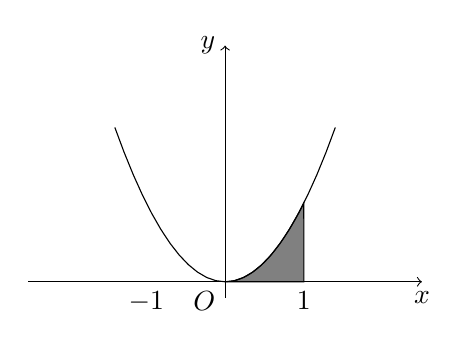
\begin{tikzpicture}
	\draw[->](-2.5,0)--(2.5,0)node[below]{$x$};
	\draw[->](0,-0.2)--(0,3)node[left]{$y$};
	\node[below left]at(0,0){$O$};
	\draw[fill=gray,domain=0:1] (0,0) -- plot({\x},{(\x)^2}) -- (1,0) -- cycle;
	\draw[domain=-1.4:1.4] plot({\x}, {(\x)^2});
	\node[below]at(1,0){$1$};
	\node[below]at(-1,0){$-1$};
\end{tikzpicture}

\end{document}

  \caption{square}\label{fig:square}
\end{figure}

如\cref{fig:square}, 对于这样的抛物线, 大家最熟悉不过了, 但如图所示的阴影面积怎么求呢?
自古希腊人发现抛物线以后, 这个问题长时间困扰着数学家们.
直到微积分的发明才使这个问题有了系统的解法.

先看不用微积分的解法:
我们先给出一个公式:

\[
  1^{2}+2^{2}+3^{2}+\ldots + n^{2} = \frac{n(n+1)(2n+1)}{6}
.\]

\begin{proof}
  对于数列 $\{a_{n}\} $, $a_n = (n+1)^{3}- n ^{3} = 3n^{2}+3n+1$
  \begin{align}
    \sum_{i=1}^{n} a_n & = (n+1)^{3}-1                                     \\
    & = 3 \sum_{i=1}^{n} i^{2} + 3 \sum_{i=1}^{n} i + n
  \end{align}
  \begin{equation*}
    \sum_{i=1}^{n} i^{2} = \frac{1}{3} \left[(n+1)^{3} -n -1 \right]
    - \frac{n(n+1)}{2}  = \frac{n(n+1)(2n+1)}{6}
  \end{equation*}
\end{proof}

\begin{figure}
  \centering
    \documentclass[border=3pt]{standalone}
\usepackage{tikz}
\usepackage{amsmath}
\usepackage{amssymb}
\usepackage{ctex}
\usetikzlibrary{matrix, calc, positioning}
\usepackage{pgfplots}
\pgfplotsset{compat=1.18}

\begin{document}
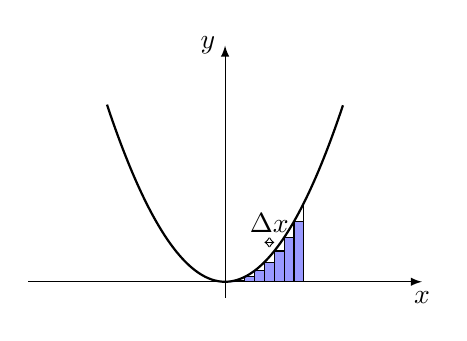
\begin{tikzpicture}[declare function={f(\x)=(\x)^(2);},
		lnode/.style={fill=white,font=\small,inner sep=0pt}]
	\newcommand*{\N}{8}
	\pgfmathtruncatemacro{\M}{\N/4}
	\coordinate (start) at (0,{f(0)});
	\foreach \X [remember=\X as \LastX (initially 0)] in {1,...,\N}
		{
			\draw[fill=blue!40!white] (\LastX/\N,0) rectangle (\X/\N,{f(\LastX/\N)});
			% \draw[red,fill=red] (1+\LastX*4/\N,{f(1+\LastX*4/\N)}) circle (2pt) ;
			\path  (\LastX/\N,0pt) coordinate (x\X);
		}
	\coordinate (end) at (1,{f(1)});
	\draw (1,0)--(1,{f(1)});
	\draw [-latex] (-2.5,0) -- (2.5,0) node (xaxis) [below] {$x$};
	\draw [-latex] (0,-0.2) -- (0,3) node [left] {$y$};
	\draw[domain=-1.5:1.5,samples=200,variable=\x,-,thick] plot ({\x},{f(\x)});
	\draw[<->] (x5|- 0,1/2)--(x6|- 0,1/2) node[above, midway] {$\Delta x$};
\end{tikzpicture}

\end{document}

  \caption{矩形逼近} \label{fig:rect}
\end{figure}

下面回归正题,
如 \cref{fig:rect}, 我们把 $y=x^{2} $ 中 $[0, 1]$ 部分分成$n$个矩形,
每条矩形的底边为 $ \frac{1}{n} = \Delta x $.

对于第$i$个矩形, 由于其前方有$i-1$个矩形,
故其高为 $h_i = f(i \Delta x) = \frac{i^{2}}{n^{2} } $.
这$n$个矩形的面积和为
\begin{align*}
  S & = \sum_{i=1}^{n} \Delta x \cdot h_i  \\
  & = \frac{1}{n^3} \sum_{i=1}^{n} i^{2} \\
  & = \frac{n(n+1)(2n+1)}{6n^3 }
\end{align*}

当$n \to +\infty$时,
这$n$个矩形的面积和可近似认为是 $f(x) = y = x^{2},x\in [0, 1] $ 与X轴围成的面积.
而
\[
  \lim_{n \to \infty} \frac{n(n+1)(2n+1)}{6n^3 } = \frac{1}{3}
.\]

故面积$ S = \frac{1}{3}$.

但这样做法十分麻烦, 况且如果不是二次函数, 在矩形面积求和时, 便会遇到障碍.
若此题用积分做, 则有
\[
  \int_{0}^{1} x^{2} \dif x= \frac{1}{3}
.\]
\begin{definition}[积分]
  若 $F'(x) = f(x)$, 则 $\int f(x) \dif x = F(x)$, 其中 「$\int $」 为积分号,
  $f(x)$称为被积函数, 「$\dif x$」称为微分算子, $F(x)$称为原函数.
\end{definition}
显然积分是求导的逆运算.

由导数的运算法则, 不难看出积分有以下法则:
\begin{enumerate}

  \item \label{law1} 若 $\int f(x) \dif x = F(x)$, 则 $\int  f(x) \dif x
    = F(x) + C$. $C = \mathrm{Constant} $(任意常数).
  \item $\int [f(x) \pm g(x)] \dif x = \int f(x) \dif x \pm \int g(x) \dif x$
  \item $\int \lambda f(x) \dif x = \lambda \int f(x) \dif x$,
    其中$\lambda $为任意常数.

\end{enumerate}

注意由\cref{law1} 法则可以知道, 一个函数有无数个原函数,
但任意两个函数之差为常数.

且对于形如 $\int f(x)g(x) \dif x,\quad \int \frac{f(x)}{g(x)} \dif x$ 这样的积分无法直接计算.

下面我们来计算一些函数的积分:
\begin{align*}
  \int x^{2} \dif x  & = \frac{1}{3} x ^3 +C \\
  \int \cos x \dif x & = \sin x + C
\end{align*}

事实上, 像导数表一样, 积分的运算也有积分表.

\[
	\int k \, \dif x           = kx + C
	.\]
\[
	\int x^n \, \dif x         = \frac{x^{n+1}}{n+1} + C \quad (n \neq -1)
	.\]
\[
	\int \frac{1}{x} \, \dif x = \ln|x| + C
	.\]
\[
	\int e^x \, \dif x         = e^x + C
	.\]
\[
	\int a^x \, \dif x         = \frac{a^x}{\ln a} + C \quad (a > 0, a \neq 1)
	.\]
\[
	\int \sin x \, \dif x      = -\cos x + C
	.\]
\[
	\int \cos x \, \dif x      = \sin x + C
	.\]
\[
	\int \tan x \, \dif x      = -\ln|\cos x| + C
	.\]


上述公式的证明, 由 求导法则 易证.

看到这里你可能会疑惑, 为什么要用$\int \,\dif x$这两个符号表示积分呢?
下面介绍另一个概念---微分.

\begin{figure}[ht]
  \centering
    \documentclass[border=3pt,tikz]{standalone}
\usepackage{tikz}
\usepackage{amsmath}
\usepackage{amssymb}
\usepackage{ctex}
\usetikzlibrary{matrix, calc, positioning}
\begin{document}
\providecommand*{\N}{6}
\renewcommand*{\N}{6}
\begin{tikzpicture}[scale=1.2,declare function={f(\x)=((0.12)*(\x)^(3)-0.9*(\x)^(2)+2.2*\x+0.8;},
		lnode/.style={fill=white,font=\normalsize,inner sep=0pt,text height=1.5em}]
	\pgfmathtruncatemacro{\M}{\N/4}
	\coordinate (start) at (.8,{f(.8)});
	\coordinate (end) at (5.05,{f(5.05)});
	\draw (4,{f(4)})--(5,{f(4)}) node[below,midway, lnode] {$\mathrm{d} x$};
	\draw (5,{f(4)})--(5,{f(5)}) node[right, midway] {$\mathrm{d} y$};
	\draw (4,{f(4)})--(5,{f(5)}) ;
	\draw [-latex] (-0.5,0) -- (6,0) node (xaxis) [below] {$x$};
	\draw [-latex] (0,-0.5) -- (0,5) node [left] {$y$};
	\draw[domain=0.5:5.2,samples=200,variable=\x,-,thick] plot ({\x},{f(\x)});
	% \draw[<->] (x2|- 0,{f(\x)-1/2})--(x3|- 0,{f(\x)-1/2}) node[above,midway] {$\Delta x$};
\end{tikzpicture}
\end{document}

    \caption{微分近似}\label{fig:simdx}
\end{figure}

由\cref{fig:simdx}, 当 $\Delta x \to 0$时,
我们记 $\Delta y = f(x+\Delta x) - f(x)$为$f(x)$在点$x$处的微分.
此时我们记$\dif y = \dif f(x) = \lim_{\Delta x \to 0} \Delta y $, $\dif x
= \lim_{\Delta x\to 0} \Delta x$,
由导数的定义式, 我们有
\begin{align}
  \frac{\dif y}{\dif x} & = \frac{f(x+\dif x) - f(x)}{\dif x} = f'(x)
  \label{eqn:directive}                                               \\
  \dif y                & = f'(x) \dif x \label{eqn:dydx}
\end{align}

\begin{note}[微分近似] \label{note:simdx}
  注意\cref{fig:simdx}, 从几何意义上来理解, 这里的$\dif y = f'(x) \dif x $就是说,
  当一个曲线上两点间距离足够近时, 我们可以用这一点的切线的变化量
  $f'(x) \dif x $去近似这条曲线的变化量 $\dif y$.
\end{note}

基于\cref{eqn:directive,eqn:dydx}, 我们可以知道微分的运算法则
\begin{align}
  \dif C                           & = 0
  \\
  \dif [ \lambda f(x) + \mu g(x) ] & = \lambda f'(x) \dif x + \mu
  g'(x) \dif x \label{eqn:linearity}                                \\
  \dif f(x)                        & = \dif [f(x)+C] = f'(x) \dif x
\end{align}

结合前面积分的定义, 对于$F'(x) = f(x)$ 有,
\[
  \int f(x) \dif x = F(x) + C
.\]
又有
\[
  f(x) \dif x = \dif[F(x) +C]
.\]
于是
\[
  \int \dif [F(x) +C] = F(x)+C
.\]

从中可以看出 $\int \text{与} \dif $连用可以相互抵消
\footnote{
  编者注:$\Delta x \to 0$ 时记为$\dif x$,
  历史上$\int $其实是$\sum_{i}^{\infty}$的简写(因为它写起来太麻烦了).
  从几何意义上来理解,
  $\int f(x) \dif x = \lim_{\Delta x \to 0} \sum_{i}^{\infty} f'(x_i)
  \cdot \Delta x_i$
  就是将每一点$x_i$函数的增量$\Delta y$都用 \cref{note:simdx}中提到的微分近似去替代,
  无限段增量累加, 便是原函数的变化量. 这也可以从几何上解释\emph{牛顿--莱布尼兹定理}.
},
即积分是微分的逆运算.

下面请读者利用以上知识证明以下等式:
\begin{align}
  \int \dif f(x)                              & = f(x)+C
  \\
  \int f(x) \dif g(x)                         & = \int f(x)g'(x) \dif
  x                                                                   \\
  \int  f(x) \dif g(x) + \int  g(x) \dif f(x) & = f(x) \cdot g(x) +C
  \label{eqn:fxgx'}
\end{align}

讲了这么多, 这和计算抛物线下面积有什么关系呢?
事实上, 我们有如下的\textbf{牛顿--莱布尼兹定理}.

\begin{theorem}[牛顿--莱布尼兹定理]
  对于 $F'(x) = f(x)$,
  \[
    \int _{a} ^{b} f(x) \dif x = F(b) - F(a)
  .\]
\end{theorem}

(编者注:从几何意义上来说)$\int _a^b f(x) \dif x$ 表示 $f(x)$在 $[a,b]$上与$x$轴围成的\emph{有向面积}
\footnote{编者注:这里「有向」二字为编者补充, $b>a>0,\And f(x)>0$ 时, $I = \int _a ^b
  f(x) \dif x >0$,
其中积分号下方的$a$称为\emph{积分下限}, 积分号上方$b$称为\emph{积分上限}, 交换积分上下限, 结果为$-I$}.

当 $f(x)$ 在 $[a,b]$ 上$>0$ 时, $\int _a ^{b} f(x) \dif x $为正值.
当 $f(x)$ 在 $[a,b]$ 上$<0$ 时, $\int _a ^{b} f(x) \dif x $为负值.

下面我们来证明$f(x)> 0,x \in [a,b]$的情形.

\begin{figure}[htbp]
  \centering
    \documentclass[border=3pt,tikz]{standalone}
\usepackage{tikz}
\usepackage{amsmath}
\usepackage{amssymb}
\usepackage{ctex}
\usetikzlibrary{matrix, calc, positioning}
\begin{document}
\providecommand*{\N}{6}
\renewcommand*{\N}{6}
\begin{tikzpicture}[scale=1.2,declare function={f(\x)=((0.12)*(\x)^(3)-0.93*(\x)^(2)+1.6*\x+2.3;},
		lnode/.style={fill=white,font=\normalsize,inner sep=0pt,text height=1.5em}]
	\pgfmathtruncatemacro{\M}{\N/4}
	\coordinate (start) at (.8,{f(.8)});
	\foreach \X [remember=\X as \LastX (initially 0)] in {1,...,\N}
	{\draw[fill=orange!40!white] (1+\LastX*4/\N,0) rectangle (1+\X*4/\N,{f(1+\LastX*4/\N)});
	% \draw[red,fill=red] (1+\LastX*4/\N,{f(1+\LastX*4/\N)}) circle (2pt) ;
	\path  (1+\LastX*4/\N,0pt) coordinate (x\X);
	\ifnum\X=1
		\draw (1+\LastX*4/\N,3pt) -- (1+\LastX*4/\N,0pt) coordinate (x\X)
		node[anchor=north east,xshift=2pt,lnode]  {$a=x_{\X}$};
	\else
		\pgfmathtruncatemacro{\itest}{mod(\X,\M)}
		\ifnum\itest=0
			\pgfmathsetmacro{\dist}{4-\LastX*4/\N}
			\ifdim\dist cm>5pt
				\draw (1+\LastX*4/\N,3pt) -- (1+\LastX*4/\N,0pt)
				node[anchor=north,lnode] {$x_{\X}$};
			\fi
		\fi
	\fi
	}
	\coordinate (end) at (5.05,{f(5.05)});
	\draw (5,3pt) -- (5,0pt)
	node[anchor=north west,xshift=-2pt,lnode]{$b=x_n$};
	\draw (5,0)--(5,{f(5)});
	\draw [-latex] (-0.5,0) -- (6,0) node (xaxis) [below] {$x$};
	\draw [-latex] (0,-0.5) -- (0,5) node [left] {$y$};
	\draw[domain=0.5:5.2,samples=200,variable=\x,red,-,thick] plot ({\x},{f(\x)});
	\draw[<->] (x2|- 0,-1)--(x3|- 0,-1) node[above,midway] {$\Delta x$};
\end{tikzpicture}
\end{document}

  \caption{a到b的矩形逼近}\label{fig:absim}
\end{figure}

如\cref{fig:absim}, 把这个不规则图形分为$n$个矩形,
每个矩形的底 $\dif x = x_n - x_{n-1} =\frac{b-a}{n}$,
对于第$i$个矩形, 其高

\begin{align*}
  h_i & = f(a+ i \cdot \frac{b-a}{n}) \\
  & = f(a+ i \dif x)
\end{align*}

\begin{align*}
  S_i & = \dif x \cdot f(a+i \dif x)         \\
  & = \dif F(a+i\dif x)                  \\
  & = F(a+ i \dif x) - F(a+(i-1) \dif x)
\end{align*}

总面积

\begin{align*}
  \sum_{i=1}^{\infty} S_i  = F(a+\dif x ) - F(a) + F(a+2 \dif x -
  F(a+\dif x )) +\ldots \\
  + F(a+n\dif x) - F(a+ (n-1)\dif x)
  \notag                \\
  = F(a+n \dif x) - F(a)
\end{align*}

又因为
\[
  n\dif x = b-a
.\]
故
\[
  \sum_{i=1}^{\infty} S_i = \int _a^{b} f(x) \dif x = F(b) - F(a)
.\]
小于零的情况同理, 至于积分的一般方法与应用请见下一节.

\paragraph{注}
这里对积分的讨论是相对粗略的极不严谨的, 对于微积分如果要严谨讨论,
我们需要讨论极限的存在准则,
实数集的完备性, 函数的两类间断点, 连续性, 可导性, 可积性以及$\epsilon \text{-} \delta $语言等.
感兴趣的同学可以自行查阅资料, 这里限于篇幅无法详细解读.

\section{积分技巧及微积分的应用}
上一节我们介绍了微积分的一些基本概念. 现在我们来讲积分的技巧及应用.

\subsection{积分技巧}
请熟知 \cref{eqn:fxgx'}.
\subsubsection*{换元法}
换元法分两类, 一类是令$x = \varphi (t)$使得$\int f(x)\dif x $转化为$\int
f\left[\varphi (t)\right] \cdot \varphi '(t) \dif t$的形式,
最后再令 $t = \varphi ^{-1} (x) $.
另一类换元法是令$t=\Phi (x)$, 转化与前者类似, 最后将结果中的$t$代换成$\Phi (x)$.

不管哪种方法, 其核心是找到一个与$x$相关的变量$t$, 对$t$进行积分, 再将$x$代回结果中.

\begin{example}
  \[
    I = \int \sqrt{1-x^{2} } \dif x, 0 \leq x \leq 1
  .\]

  它的原函数我们注意力不够, 看不出来.

  不妨令$x = \cos t,t \in \left[0,\frac{\pi}{2} \right]$
  则原积分
  \begin{align*}
    I & = \int  \sin t \dif \cos t                        \\
    & = - \int \sin ^{2} t \dif t                       \\
    & = \int \frac{ \cos 2t }{2} \dif t - \frac{1}{2} t
  \end{align*}

  再令$\mu  = 2t$, 则
  \begin{align*}
    \int \frac{\cos 2t}{2}\dif t & = \int \frac{\cos  \mu}{2} \dif
    \frac{\mu}{2}                                                       \\
    & = \frac{1}{4} \int \cos \mu \dif \mu \\
    & = \frac{1}{4} \sin \mu               \\
    & = \frac{1}{4} \sin  2t + C
  \end{align*}

  故原积分
  \begin{align*}
    I & = \frac{1}{4} \sin  2t - \frac{1}{2}t +C                    \\
    & = \frac{1}{4} \sin 2(\arccos x ) - \frac{1}{2} \arccos x +C
  \end{align*}
  其中$\arccos x$表示$\cos x$的反函数.
\end{example}

\subsubsection*{分部积分法}
由恒等式
\[
  \int f(x)\dif g(x) + \int g(x) \dif f(x) = f(x)\cdot g(x)
.\]
可以导出以下积分技巧:
对于$\int f(x)g(x) \dif x$型积分, 令$F'(x) = f(x)$, $G'(x) = g(x)$, 则
\begin{align*}
  \int f(x)g(x) \dif x & = G(x)f(x) - \int G(x) \dif f(x) \\
  & = F(x)g(x) - \int F(x) \dif g(x)
\end{align*}
两个等式, 哪个方便用哪个.

\begin{example}
  \begin{align*}
    \int x \sin x\dif x & = - \int x \dif \cos x                          \\
    & = -\left(x \cos x - \int  \cos x \dif x \right) \\
    & = \sin x - x \cos x +C
  \end{align*}
\end{example}
别忘了, $\int \dif$  的常数可以直接提出来, 参见 \cref{eqn:linearity}.

\subsection{积分的应用}
本节主要涉及定积分, 若一个函数的不定积分可求, 则其求定积分易如反掌.

\subsubsection{圆锥体积推导}

如 \cref{fig:circular_cone}, 高$PO = h$, 底面积$S$, 在$PO$上取一点$M$,
作平行于底面的截面$\odot M$, 记$PM = x$, 则
\[
  S_m = \frac{x^{2}}{h^{2} } \cdot S
.\]

过点$M$ 作一段无穷小的高$\dif x$.
则
\[
  \frac{x^{2}}{h^{2} }\cdot S \cdot \dif x = \dif V
.\]

\begin{figure}[htbp]
  \centering
    \begin{subfigure}{0.45\textwidth}
      \centering
      \documentclass[12pt,tikz]{standalone}
\usepackage{xcolor}
\usepackage{tikz}
\usepackage{tikz-3dplot}

\begin{document}
\pgfmathsetmacro\th{65}
\pgfmathsetmacro\az{110}
\tdplotsetmaincoords{\th}{\az}
%parameters of the cone
\begin{tikzpicture}[scale=1, tdplot_main_coords, axis/.style={blue,thick}]
	\pgfmathsetmacro\R{2} %radius of base
	\pgfmathsetmacro\v{5} %height of cone
	\pgfmathsetmacro\M{3}
	\path (0,0,0) coordinate (O)
	(0,0,\M) coordinate (M)
	(0,0,\v) coordinate (P);
	\foreach \point/\pos in {P/above, O/below, M/left}
		{\fill (\point) circle[radius=1pt] node[\pos] {$\point$};}
	\draw[dashed] (P) -- (O);

	\pgfmathsetmacro\RM{\R - \M*\R/\v}

	\pgfmathsetmacro\cott{{cot(\th)}}
	\pgfmathsetmacro\fraction{\R*\cott/\v}
	\pgfmathsetmacro\fraction{\fraction<1 ? \fraction : 1}
	\pgfmathsetmacro\angle{{acos(\fraction)}}

	% % angles for transformed lines
	\pgfmathsetmacro\PhiOne{180+(\az-90)+\angle}
	\pgfmathsetmacro\PhiTwo{180+(\az-90)-\angle}

	% % coordinates for transformed surface lines
	\pgfmathsetmacro\sinPhiOne{{sin(\PhiOne)}}
	\pgfmathsetmacro\cosPhiOne{{cos(\PhiOne)}}
	\pgfmathsetmacro\sinPhiTwo{{sin(\PhiTwo)}}
	\pgfmathsetmacro\cosPhiTwo{{cos(\PhiTwo)}}

	\tdplotdrawarc[tdplot_main_coords,dashed]{(O)}{\R}{\PhiTwo}{\PhiOne}{anchor=north}{}
	\tdplotdrawarc[tdplot_main_coords,thick]{(O)}{\R}{\PhiOne}{360+\PhiTwo}{anchor=north}{}

	\tdplotdrawarc[tdplot_main_coords,dashed]{(M)}{\RM}{\PhiTwo}{\PhiOne}{anchor=north}{}
	\tdplotdrawarc[tdplot_main_coords,thick]{(M)}{\RM}{\PhiOne}{360+\PhiTwo}{anchor=north}{}

	% % displaying transformed surface of the cone (rotated)
	\draw[thick] (0,0,\v) -- (\R*\cosPhiOne,\R*\sinPhiOne,0);
	\draw[thick] (0,0,\v) -- (\R*\cosPhiTwo,\R*\sinPhiTwo,0);
\end{tikzpicture}
\end{document}

      \caption{$M$点截面}\label{fig:circular_cone}
    \end{subfigure}
    \begin{subfigure}{0.45\textwidth}
      \centering
      \documentclass[12pt,tikz]{standalone}
\usepackage{xcolor}
\usepackage{tikz}
\usepackage{tikz-3dplot}

\begin{document}
\pgfmathsetmacro\th{65}
\pgfmathsetmacro\az{110}
\tdplotsetmaincoords{\th}{\az}
%parameters of the cone
\begin{tikzpicture}[scale=1, tdplot_main_coords, axis/.style={blue,thick}]
	\pgfmathsetmacro\R{2} %radius of base
	\pgfmathsetmacro\v{5} %height of cone
	\pgfmathsetmacro\M{3}
	\path (0,0,0) coordinate (O)
	(0,0,\M) coordinate (M)
	(0,0,\v) coordinate (P);
	\foreach \point/\pos in {P/above, O/below, M/left}
		{\fill (\point) circle[radius=1pt] node[\pos] {$\point$};}
	\draw[dashed] (P) -- (O);

	\pgfmathsetmacro\RM{\R - \M*\R/\v}

	% \draw[thick,->] (0,0,0) -- (1,0,0) node[anchor=north east]{$x$};
	% \draw[thick,->] (0,0,0) -- (0,1,0) node[anchor=north west]{$y$};
	% \draw[thick,->] (0,0,0) -- (0,0,1) node[anchor=south]{$z$};

	\pgfmathsetmacro\cott{{cot(\th)}}
	\pgfmathsetmacro\fraction{\R*\cott/\v}
	\pgfmathsetmacro\fraction{\fraction<1 ? \fraction : 1}
	\pgfmathsetmacro\angle{{acos(\fraction)}}

	% % angles for transformed lines
	\pgfmathsetmacro\PhiOne{180+(\az-90)+\angle}
	\pgfmathsetmacro\PhiTwo{180+(\az-90)-\angle}

	% % coordinates for transformed surface lines
	\pgfmathsetmacro\sinPhiOne{{sin(\PhiOne)}}
	\pgfmathsetmacro\cosPhiOne{{cos(\PhiOne)}}
	\pgfmathsetmacro\sinPhiTwo{{sin(\PhiTwo)}}
	\pgfmathsetmacro\cosPhiTwo{{cos(\PhiTwo)}}

	\tdplotdrawarc[tdplot_main_coords,dashed]{(O)}{\R}{\PhiTwo}{\PhiOne}{anchor=north}{}
	\tdplotdrawarc[tdplot_main_coords,thick]{(O)}{\R}{\PhiOne}{360+\PhiTwo}{anchor=north}{}

	\tdplotdrawarc[tdplot_main_coords,dashed]{(M)}{\RM}{\PhiTwo}{\PhiOne}{anchor=north}{}
	\tdplotdrawarc[tdplot_main_coords,thick]{(M)}{\RM}{\PhiOne}{360+\PhiTwo}{anchor=north}{}

	% % displaying transformed surface of the cone (rotated)
	\draw[thick] (0,0,\v) -- (\R*\cosPhiOne,\R*\sinPhiOne,0);
	\draw[thick] (0,0,\v) -- (\R*\cosPhiTwo,\R*\sinPhiTwo,0);
	\pgfmathsetmacro\N{1}

	\foreach \X [remember=\X as \LastX (initially 0)] in {0, \N,...,\v}
		{
			\path (0,0,\X) coordinate (X);
			\path (0,0,\LastX) coordinate (L);
			\pgfmathsetmacro\RX{\R - \X*\R/\v}
			\pgfmathsetmacro\RLX{\R - \LastX*\R/\v}

			\tdplotdrawarc[tdplot_main_coords]{(X)}{\RX}{\PhiOne}{360+\PhiTwo}{anchor=north}{};
			\tdplotdrawarc[tdplot_main_coords]{(L)}{\RX}{\PhiOne}{360+\PhiTwo}{anchor=north}{};

			\tdplotdrawarc[tdplot_main_coords,dashed]{(X)}{\RX}{\PhiTwo}{\PhiOne}{anchor=north}{}

			\pgfcoordinate{edge1_top}{ \pgfpointcylindrical{\az}{\RX}{\X} };
			\pgfcoordinate{edge1_bottom}{ \pgfpointcylindrical{\az}{\RX}{\LastX} };
			\draw(edge1_top) -- (edge1_bottom);

			\pgfcoordinate{edge2_top}{ \pgfpointcylindrical{\az+180}{\RX}{\X} };
			\pgfcoordinate{edge2_bottom}{ \pgfpointcylindrical{\az+180}{\RX}{\LastX} };
			\draw (edge2_top) -- (edge2_bottom);

			\ifnum\X=3
				\pgfcoordinate{dxtop}{ \pgfpointcylindrical{\az+180}{\RX+0.5}{\X} };
				\pgfcoordinate{dxbot}{ \pgfpointcylindrical{\az+180}{\RX+0.5}{\LastX} };
				\draw[dashed] (dxtop)--(edge2_top)
				(dxbot) -- (edge2_bottom);
				\draw[<->] (dxtop)--(dxbot) node[anchor=east,midway, xshift=-5pt]  {$\mathrm{d}x$};
			\else
				\draw (edge2_top) -- (edge2_bottom);
			\fi

			% \ifnum\X=0
			% 	\draw (\LastX/\N,3pt) -- (\LastX/\N,0pt) coordinate (x\X)
			% 	node[anchor=north east,xshift=2pt,lnode]  {$a=x_{\X}$};
			% \else
			% 	\pgfmathtruncatemacro{\itest}{mod(\X,\M)}
			% 	\ifnum\itest=0
			% 		\pgfmathsetmacro{\dist}{1-\LastX/\N}
			% 		\ifdim\dist cm>9pt
			% 			\draw (\LastX/\N,3pt) -- (\LastX/\N,0pt)
			% 			node[anchor=north,lnode] {$x_{\X}$};
			% 		\fi
			% 	\fi
			% \fi
		}

\end{tikzpicture}
\end{document}

      \caption{用小圆柱逼近体积}\label{fig:circular_sim}
    \end{subfigure}
    \caption{圆锥示意图}
\end{figure}

如\cref{fig:circular_sim}, 我们可以用无数个小圆柱的体积去逼近圆锥的体积, 当每个圆柱的高足够小, 体积就足够精确.

\begin{align*}
  V & = \int _0^{h} \frac{S}{h^{2} }\cdot x^{2} \dif x         \\
  & = \frac{S}{h^{2} }\int _0^{h} x^{2}\dif x                \\
  & = \frac{S}{h^{2}} \cdot \left(\frac{1}{3} h^3 -0 \right) \\
  & = \frac{1}{3} Sh
\end{align*}

\subsubsection{变力做功}
我们知道, 当$\vec{F} $为恒力时, $W = \vec{F} \cdot \vec{x} $.
若$\vec{F} $为变力, 我们就需要找到$\vec{F} $与$\vec{x} $的函数关系, 便可用积分解决变力做功问题.

\begin{figure}
  \centering
    \documentclass[border=5pt,tikz]{standalone}
\usepackage{tikz}
\usepackage{amsmath}
\usepackage{amssymb}
\usepackage{ctex}
\usetikzlibrary{matrix, calc, positioning}
\usepackage{pgfplots}
\pgfplotsset{compat=1.18}

\begin{document}

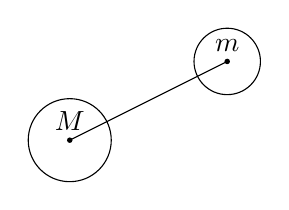
\begin{tikzpicture}
	\draw (0,0) circle [radius = 15pt] node[above] {$M$}
	(2,1) circle [radius=12pt] node[above] {$m$};
	\fill (0,0) circle[radius=1pt]
	(2,1) circle[radius=1pt];
	\draw (0,0) -- (2,1);

\end{tikzpicture}

\end{document}

  \caption{质量分别为$M,m$的星体}\label{fig:planet}
\end{figure}

\begin{example}
  两者皆可看作质点.
  若两星体由于引力而逐渐沿中心连线相互靠近,
  我们以$M$为参考系, 视作不动.
  当两者距离由$H$ 变化到 $h \, (H>h)$时, 引力做了多少功?

  我们知道, 当二者相距$x$时, 有
  \[
    F = \frac{GMm}{x^2}
  .\]

  \begin{figure}[ht]
    \centering
      \documentclass[border=3pt]{standalone}
\usepackage{tikz}
\usepackage{amsmath}
\usepackage{amssymb}
\usepackage{ctex}
\usetikzlibrary{matrix, calc, positioning}
\usepackage{pgfplots}
\pgfplotsset{compat=1.18}

\begin{document}

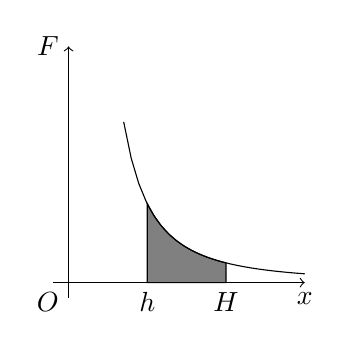
\begin{tikzpicture}
	\draw[->](-0.2,0)--(3,0)node[below]{$x$};
	\draw[->](0,-0.2)--(0,3)node[left]{$F$};
	\node[below left]at(0,0){$O$};
	\draw[fill=gray,domain=1:2] (1,0) -- plot({\x},{1/(\x)^2}) -- (2,0) -- cycle;
	\draw[domain=0.7:3] plot({\x}, {1/(\x)^2});
	\node[below]at(1,0){$h$};
	\node[below]at(2,0){$H$};
\end{tikzpicture}

\end{document}

    \caption{$F$-$x$图像}\label{fig:Fx}
  \end{figure}

  如\cref{fig:Fx}, 显然有$W_{Hh}$为阴影部分面积.
  \begin{align*}
    W_{Hh} & = \int _{h} ^{H} \frac{GMm}{x^2} \dif x    \\
    & = GMm \left(\frac{1}{h}-\frac{1}{H}\right)
  \end{align*}

  \paragraph{引力势能}
  实际上,任意保守场都具有一个势能函数,
  我们将无穷远处的引力势能视为$0$,
  则某点的重力势能等于物体从无穷远点运动到该点时,引力所做的功。即
  \[
    E_{\mathrm{p}} = \int_r^\infty \frac {GMm} {x^2} \dif x=\frac {GMm}r
  .\]

  对于两点电荷之间的电场力同理.

\end{example}

\chapter{电容定义式}

首先所谓的\emph{高斯定理}:
\[
  \oint_{\mathcal S} \vec{E}(\vec{r})\cdot \dif \vec{s} =
  \frac{Q}{\epsilon_0} = \frac{1}{\epsilon_0} \int_{\mathcal S}
  \rho(\vec{r}) \dif V ~
.\]

看不懂,没关系。简单来讲就是我们在空间上画一个\emph{闭合曲面}(例如我们取个球面),
如果一个点电荷在这个球外面,那么我们都知道有的电场线如果穿进这个球,那么它们也必定会穿出这个球,
所以穿进去和穿出去的电场线必定相等的,这个说法不太严谨。
我们学磁学时候学过法拉第电磁感应定律里面有个概念叫\emph{磁通量},这里也一样,就是电场强度 $E$ 和面积
$S$的乘积(虽然实际是积分,但是我们都可以意会)。$ES$ 就是电通量(磁通量
$\phi=BS$,是不是很像)。也就是说如果这个球里面没有点电荷,那么净通量就是
$0$(进去的等于出去的)。而如果球里面有正电荷呢,那出去的就应该比进去的多。也就是说我们得到一个重要结论:

对于封闭曲面,净通量=源的强度。

高斯定理定性分析其实就是这么一回事。特殊的,如果我们有一个点电荷 $Q$
位于一个球的球心位置,那么球面上由于对称,电场强度处处大小相等。所以 $E$ 不变,那么净通量就是 $ES$,那源强度应该跟电荷量 $q$
成正比。那么具体公式是什么呢,答案是

$$
ES=\frac{Q}{\epsilon_0}
$$

可能有的同学对这个公式很陌生,那么我们不妨推导一下,球的面积

$$
S=4\pi r^2
$$

$$
E=\frac{Q}{4\pi r^2 \epsilon_0}
$$

我们令 $k=\frac{1}{4\pi \epsilon_0}$,因为这玩意都是常数。然后得到

$$
E=k\frac{Q}{r^2}
$$

我们给 $k$ 取了个名字叫库伦常数,是不是突然想起来这是什么了,这不就是\emph{点电荷电场强度公式}吗。所以高斯定理讲的就是电通量和电荷量的比例关系。

$$
ES=\frac{Q}{\epsilon_0}
$$

这个 $\epsilon_0$ 叫真空介电常数,物理含义很明显吧,就是个比例系数。
那么回到电容这里,我们知道电容定义 $C=\frac QU$。
也就是说如果我能用 $Q$ 表示出来 $U$ 多大是不是就解决了。
刚才 $ES=\frac{Q}{\epsilon_0}$,我们还知道 $Ed=U$ ,所以

$$
U=Ed =\frac{Q}{S\cdot \epsilon_0} \cdot d
$$

$$
C=\frac{Q}{U}=\frac{ES\cdot
\epsilon_0}{Ed}=\frac{S\cdot\epsilon_0}{d}=\frac{S}{4\pi kd}
$$

我们发现现在跟书上给的就差了一个 $\epsilon_r$,这又是什么玩意呢,原理是我们刚才用到的 $\epsilon_0$
那个是真空条件下的。如果你中间介质不是真空的还要再多乘一个比例系数$\epsilon_r$,我们刚才算的那个 $C$ 是 $C_0$,实际
$C=\epsilon_r\cdot C_0$。也就是

$$
C=\frac{\epsilon_r \cdot S}{4\pi k}
$$

\chapter{``$\mathrm{e}$''的起源}

1727 年,欧拉刚满 20 岁,这时候他研究生毕业,找不到工作
(是的,在当时高斯、黎曼、爱因斯坦等人也找不到工作).
不过欧拉的好朋友 丹尼尔\textperiodcentered 伯努利 在俄罗斯圣彼得堡科学院当教导主任,
于是欧拉就去医学院当生理卫生老师(魏尔斯特拉斯 都当过体育老师,所以从源头上说,我们的数学不是生理卫生老师教的就是体育老师教的🤣)
学习了两个月生理卫生课后他就跑去圣彼得堡了。
他因有工作而开心,但没有因此而忘记使他开心的数学。
他经常在下班后搞点数学玩玩,从指数函数$y=2^{x}$,
和导数的定义开始爆算。\footnote{注:当时未有极限的概念.}

\begin{align*}
  \left( 2^{x}  \right)' & = \lim_{h \to 0} \frac{2^{x+h}-2^{x} }{h} \\
  & = \lim_{h \to 0} \frac{2^{x}\cdot 2^{h}-2^{x}   }{h} \\
  & = 2^{x} \lim_{h \to 0} \frac{2^{h}-1 }{h}
\end{align*}

这样,$2^{x} $的导数变成它自己乘以一个系数。

这个系数是多少呢,欧拉硬算一下发现它约等于$0.6931$,
那$y=3^x$呢,他算了一下发现仍是一个系数约等于$1.09861$,
如果继续算下去就会发现$4$、$5$、$6$、$7$的$x$次方对应的系数
依次为$1.3862$,$1.6094$,$1.7917$,$1.9459$,
到这里欧拉发现一个有趣的问题:
我们应以怎样一个数为底其对应系数为$1$呢,换句话说,
``会不会有一个指数函数的导数等于它本身呢'',欧拉心想,那算吧:

我们先假设有这么个数$a$

\begin{align*}
  \left(a^{x}\right)' & = \lim_{h \to 0} \frac{a^{x+h}-a^{x}}{h}  \\
  & = \lim_{h \to 0} a^{x}\cdot a^{h} - a^{x} \\
  & = a^{x} \lim_{h \to 0} \frac{a^{h}-1}{h}
\end{align*}
令这个系数等于 1.

\begin{align*}
  \lim_{h \to 0} \frac{a^{h}-1}{h} &= 1 \\
  \lim_{h \to 0} a^{h} - 1 &=\lim_{h \to 0} h \\
  \lim_{h \to 0} a^{h} &=\lim_{h \to 0} h+1 \\
  a &=\lim_{h \to 0} (h+1)^{\frac{1}{h}}
  \intertext{换个元,我们就有}
  a &=\lim_{n \to \infty} (1+\frac{1}{n})^{n}
\end{align*}

于是欧拉爆算发现这个值约等于$2.71828182845904(5)$,
其实这个数在莱布尼茨时期已被发现,
后人将其称为欧拉数,即``$\upe$''.

在当时,像$\frac{\pi}{4}$这类无理数的无穷级数形式表示是热门话题,
那么\upe 的无穷级数形式是什么样的呢?

我们利用一下刚才的结论
$(\upe ^{x})' = \upe ^{x} $, 我们可以猜测一下它的无穷级数:
\begin{equation}
  e^{x}= 1+x + \frac{x^2 }{2!} + \frac{x^3}{3!} + \ldots +
  \frac{x^{n} }{n!} \label{eqn:ex}
\end{equation}

因为我们知道幂函数的求导公式$(x^{n})' = nx^{n-1}  $,
对上式求导得
\begin{align*}
  (e^{x})' &= 1' &+ x' &+ \left(\frac{x^2}{2!}\right) &+
  \left(\frac{x^3}{3!}\right)' &+ \ldots &+
  \left(\frac{x^{n}}{n!}\right)' &\quad \\
  &= 0 &+ 1 &+ x
  &+ \frac{x^2}{2!} &+ \ldots &+ \frac{x^{n-1}}{(n-1)!} &+\ldots
\end{align*}

式子整体不变,恰好满足了 $\left(\upe^{x}\right)' = \upe^{x}  $
于是乎这就是$e^{x}$的无穷级数。

带入$x=1$,得
\[
  \upe = \frac{1}{0!} + \frac{1}{1!} + \frac{1}{2!} + \ldots
.\]

(是的,这是欧拉凭空想象得来的,可见想象力多么重要🤓)
\Cref{eqn:ex} 实际上就是$\upe ^{x} $在$x=0$处的泰勒展开。

\chapter{碰撞的物块与圆周率:一场奇妙的物理之旅}

物体的碰撞和圆周率,这两者看起来似乎毫无关系,但在一次巧合之中,科学家们发现了他们之间的关联,令人惊讶。

假定在一个无摩擦的平面上有 2
个小物块,左侧的方块初始$v_{2}=0$,质量$m_{2}$小于等于右侧物块$m_{1}$,右侧物块则以一定的速度$v_{1}$向左运动,两个方块会互相碰撞,设为弹性碰撞,他们左边有一堵墙。
那么在这么一个系统之内,他们总共会发生多少次碰撞(包括左侧物块与墙壁的碰撞)呢?

有一个特别重要的思想,就是从特殊到一般。

让我们先假定两个物块质量$m_{1}=m_{2}=\SI{1}{\kg}$.
那么很明显,由于他们之间发生了弹性碰撞,且无内能的转化,
由物理必修课本中的机械能守恒有
\[
  \frac{1}{2} m_{1}v_{1}^2+\frac{1}{2} m_{2}v_{2}^2  =
  \frac{1}{2} m_{1}v_{1}'^2 + \frac{1}{2} m_{2}v_{2}'^2
.\]

又由选修一课本中的动量定理
\[
  m_{1}v_{1}+m_{2}v_{2}=
  m_{1}v_{1}' + m_{2}v_{2}'
.\]

我们可知,
\begin{align*}
  v_{1}' = \frac{(m_{1}-m_{2})v_{1} + 2m_{2}v_{2}}{m_{1}+m_{2}} \\
  v_{2}' = \frac{(m_{2}-m_{1})v_{2} + 2m_{1}v_{1}}{m_{1}+m_{2}}
\end{align*}

通过简单的物理计算就可以知道,其总共会碰撞 3 次。

倘若我们把右边的物块质量增大到$m_{1}=\SI{100}{\kg}$, 通过电脑的模拟计算,我们也可以知道他们总共碰撞了 31 次。

再增大一点到 \SI{10000}{\kg}, 计算得知他们总共会碰撞 314 次。
看着这些碰撞的次数,你想起了什么吗?$314$, $3.14$ ,$\pi$?
这会是一个偶然的巧合吗?那再让我们继续增大质量,增大到\SI{1000000}{\kg}, 计算机屏幕上的小物块经过多次碰撞之后,数字定格在了 3141 次。
好吧,看起来这好像并不是一个巧合,他碰撞的次数似乎与$\pi$之间有一种微妙的关系,接下来就应该一般分析了。

让我们设右侧物块的质量为$m_{1}$,左侧物块的质量为$m_{2}$.
因为能量守恒,所以我们可以写出下式:

\[
  E = \frac{1}{2} m_{1}v_{1}^2 + \frac{1}{2} m_{2}v_{2}^2
.\]

在碰撞过程中,$m_{1},m_{2},E$不变,变量有$v_{1},v_{2}$.
在数据分析的时候,借助数形结合来解答问题是较为常用的一种方法。
上式中的两个变量,我们就可以这样处理。
我们设一个点为$(x,y)$,以$v_{1}$为$x$轴,$v_{2}$为$y$轴,建立平面直角坐标系。
不妨设右侧为速度的正方向。
那么上式的形式就可以看做$ax^2+by^2=c$.
我们可以发现这一条表达式所对应的图形是椭圆\footnote{详见数学课本选择性必修一圆锥曲线一章}.

%%

但是我们的高中知识的确有限,对于椭圆的研究比较少,因此,我们无法对椭圆进行直接的研究。
为了顺利的研究这个图形,我们就可以采用数学的另一种高级方法,叫做映射。
\footnote{ 映射 (map) 是函数概念的推广,它描述了两个集合之间的关系,如果这两个集合是同一个,那么映射也称作变换。}
通过化椭圆为圆,从而将我们所学过的知识关联起来,以顺利解决这个问题。

让我们通过线性映射(即仿射变换)重新将$\sqrt{m_{1}}v_{1} $设为$x$轴,将$\sqrt{m_{2}}v_{2}
$设为$y$轴,那么我们就可以得到一个美妙的式子:$x^2+y^2=E$.
很成功地,我们将椭圆转化成了圆,接下来我们在数学工具中画出它的图形:

%%

因为$x^2$和$y^2$的和不变,
无论两个物块的初始动能为何值,它们所对应的点$\left(\sqrt{m_{1}}v_{1}, \sqrt{m_{2}}v_{2}
\right)$都在该圆上,和为$2E$. 碰撞过程可视为点在图上运动的过程。

接下来我们来考虑动量设总动量为$P$,则有:
\[
  m_{1}v_{1}+m_{2}v_{2} = P
.\]

根据上述坐标系,我们可以将上式写成:
\[
  \sqrt{m_{1}}\left( \sqrt{m_{1}}v_{1} \right) + \sqrt{m_{2}} \left(
  \sqrt{m_{2}}v_{2} \right) = P
.\]

可以看出来,这条式子所表示的是一条直线$\sqrt{m_{1}} x + \sqrt{m_{2}}y = P  $.
由于$v_{2}$初始值为$0$,所以在碰撞前,它必处于上图红点处,而且该直线的斜率为$-\sqrt{\frac{m_{1}}{m_{2}}} $.

(这里由于$m_{1},m_{2}$为变量,所以我们先随便画一条$k<0$的线)
过红点做斜率为$-\sqrt{\frac{m_{1}}{m_{2}}} $的一条直线交于圆于第二个点,该点就为第一次双物块碰撞后所处于的状态点。

让我们来分析左侧物块与墙壁的碰撞,由于该系统总动能未变,所以碰撞后点必然在圆上。
由于$v_{2}$不改变,$v_{1}$反向,所以我们只需要作出过第二个点垂直于 x
轴的一条直线,它与圆的另一个交点就是左侧物块与墙壁碰撞后,系统所处于状态点。
以此类推,我们便可以做出下图:

那么,这样的碰撞什么时候是个头呢?
我们来假设一下,若左侧物块碰撞后速度向左,那么它最后一定会与墙壁再发生碰撞,所以左侧物块最终碰撞后的速度应向右。
同理,右侧的物块速度也应向右。
若左侧物块向右的最终速度大于右侧物块向右的速度,则两个物块还会发生一次碰撞。
所以左侧物块最终末速度应当小于右侧物块的末速度,即$0< v_{2} < v_{1}$, 所以该点应当位于第一象限,
且在$v_{1}=v_{2}$所在的直线$y=\sqrt{\frac{m_{2}}{m_{1}}}x$与$x$轴围成的区域内,

我们在图中做出这条直线:

所以当点位于上图绿色区域内时 (包含边界),该系统将不会再发生碰撞,他们之间碰撞的次数可以通过数上图的线段的多少的得知。
到此,我们就把这个物理问题转化成了一个数学问题。

我们就上图进行分析,设每一条倾斜的直线的倾斜角为$\theta $,则
$\tan \theta  = -\sqrt{\frac{m_{1}}{m_{2}}} $ ,
看着上面那一个图,你会不会觉得是很规则的锯齿状?我们稍微研究一下他们的几何关系,容易发现圆上的每一段弧所对应的圆周角都是相等的
(瞪眼,平行秒啦),再而推出每一段的弧长与圆心角也是相等的。

由于绿色区域上边缘所在的直线的斜率为$\sqrt{\frac{m_{2}}{m_{1}}} $,所以其对应的倾斜角就为$\theta $.
如图不难看出,最右端的这段弧长所对应的圆心角小于等于$\theta $.
所以实际上我们就把题目上的问题转化成了:这一个圆上可以存在多少段圆心角为$2\theta$的弧
(由图像其实不难看出,圆内弦的条数与其所拥有的弧数其实是相等的,故此处不再说明)?
设在这圆上有$n$段这样的弧,那我们就可以得出来:$n \cdot 2 \theta \cdot R \le 2 \pi R$.

经过化简,我们就可以得到: $n \cdot \theta \le  \pi $,
\footnote{ 高一的新同学,请注意这用的$\theta$为弧度制单位下的角度表达,并不是在初中时常用的角度制 }
在前文中,我们猜想是$n$与$\pi $有一定的关系。
然而根据这个式子,我们并不能很好地看出来它们之间有什么样的直接关系。
让我们回到前文可以看出来,随着右侧物块的质量与左侧物块质量之比逐渐增加时,
$n$似乎在逐渐靠近$\pi $的各位数字,我们不妨把这个比值再次增大。
这时候,$\theta $的值其实在不断的减小 ($y=\tan x$ 在 $\left( - \frac{\pi}{2},0
\right) $ 上是一个增函数).

当这个比值足够大的时候,那么$\tan
\theta$的值也会逐渐变小,我们又由小角近似可知,在$\theta$足够小的时候,$\theta \approx \tan \theta $.
于是我们上面的式子可以改写成:$n \cdot \tan \theta \le  \pi $.
这个$\tan \theta$可以是多小呢?
我们假设它小到可以忽略其具体数值,只保留数量级,那么上式就可以写成:$n \cdot 10^{-q} \le  \pi  $
由于$n$是正整数,所以该式就可以理解为$q$位精确度下$\pi $的数值。

到此,他们之间关系就被我们发现了。

经过科学家们的验证,在现有计算仪器的精度下,这样子计算出来的$\pi $的近似值是较为精确的。
所以我们的证明过程也差不多结束了。

纯粹的科学家们善于从现实世界的混乱中将核心抽离出来,更深层次的原因是纯粹可以暴露隐藏的联系。
之前,格雷戈里·盖普 (Gregory Gap)
的论文,一束光在两面镜子之间以一定角度反射,最终光束反射的次数也与$\pi $有密切的关系,
该现象与数学之间的微妙关系的确令人惊叹。

在最后笔者想要告诉各位读者的是:科学的魅力在于它能够揭示看似无关的现象之间的深刻联系。
物体的碰撞次数与圆周率$\pi $之间的关系,就是一个典型的例子,展示了生活中隐藏的数学之美。
这种美不仅仅是形式上的,更是功能上的,它体现了宇宙运行的基本规律。
在探索这个现象的过程中,我们运用了物理学、数学一些相关知识。
这些知识帮助我们将复杂的问题简化,从而揭示问题的本质。
这也提醒我们,我们的学习不仅仅是记忆公式和事实,更是一种思维方式,一种解决问题的方法。
对于我们每个人来说,这些知识教会我们如何观察世界,如何思考问题,如何寻找答案。
在这个信息爆炸的时代,我们需要的不仅仅是知识,更是一种能够帮助我们理解世界的能力。
让我们保持好奇心,保持求知欲,不断探索,不断发现。
就像那些伟大的科学家一样,从看似平凡的现象中发现不平凡的真理。
只有这样,我们才能真正理解宇宙所蕴含的奥秘,才能真正享受到科学带来的乐趣。


\begin{appendices}
  \listoffigures
  \listoftables
\end{appendices}
\backmatter
\layout
\end{document}
